\subsection{Class Diagrams}

The class diagram captures the static structure of the backend: the core domain entities, their attributes, and the relationships between them. The model is organised along Domain-Driven Design lines into three packages --- \textit{Identity \& Access}, \textit{Course \& Ingestion}, and \textit{Assessment \& Interview}. The three paragraphs below state the design decision that shapes each package; the full entity listing, with attributes, cardinalities and the rationale behind each relationship, is catalogued in Appendix~\ref{appendix:class-diagram}.

\begin{itemize}
    \item \textbf{Identity \& Access.} Authorisation is \textbf{role-based, not inheritance-based}. There is a single concrete \texttt{User} entity; a person's capabilities come from rows in \texttt{user\_role\_assignments} that bind them to a \texttt{Role} at a declared scope (global, organisation, org-unit or course), and each role carries a set of \texttt{Permission} codes. Modelling ``student'' and ``teacher'' as subclasses was rejected because the same account is routinely both --- a teaching assistant enrolled on another course --- and because a scoped assignment expresses ``instructor \emph{of this course}'', which a subclass cannot.
    \item \textbf{Course \& Ingestion.} A \texttt{Course} composes \texttt{LearningMaterial}s, each of which is versioned: a \texttt{LearningMaterialVersion} references bytes held in object storage through \texttt{storage\_object\_id}, and the database stores that reference rather than the file. Each version decomposes into \texttt{DocumentChunk}s carrying a 3072-dimensional embedding, which is what the retrieval pipeline searches.
    \item \textbf{Assessment \& Interview.} Maps the path from theory validation (\texttt{QuizAttempt}) to practical application (\texttt{InterviewSession}), and how the per-question record of an interview is aggregated into a personalised \texttt{GapReport}.
\end{itemize}

\begin{figure}[H]
    \centering
    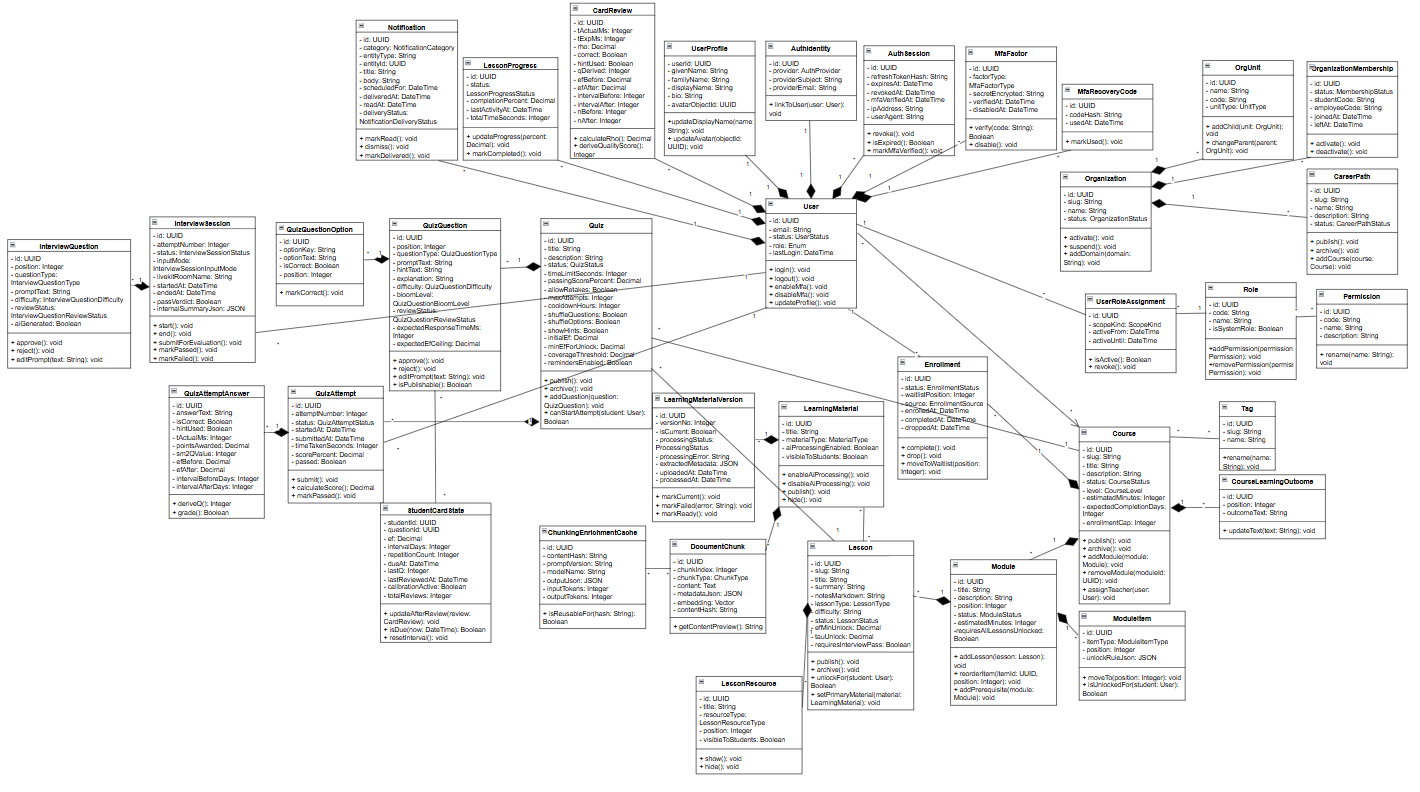
\includegraphics[width=0.95\textwidth]{graphics/class_diagram.png}
    \caption{UML Class Diagram representing the core Domain Entities of aBridgeAI}
    \label{fig:class_diagram}
\end{figure}
